\section*{System 3: Novel sEMG Device with Impaired User Study}
\setcounter{subsection}{0}
\renewcommand*{\theHsection}{chX.\the\value{section}}
\subsection{Surface EMG Recording}
\label{sec:semg_hardware}
We found a number of practical issues with the Emotiv Epoc as an input device. The two most important were the impracticality of the form bulky factor of the device and the difficulty of configuring and maintaining its electrodes to work correctly. To address some of these issues, we adopted a novel input device under development at UC Davis which is designed to be used by severely impaired individuals. This device has an extremely noninvasive profile, requiring only a single sEMG recording site behind the ear. 

The muscles behind the ear are are innervated by nerves that come directly from the brain stem, without ever entering the spine. Even individuals with the most severe spinal cord paralysis can still access these muscles. Although some individuals are able to independently move their ears, we have found that even individuals that cannot move their ears can learn to activate the muscles in that region without achieving overt motion when they are given visual feedback. This activation produces signals that can be detected by electrodes mounted on the surface of the skin. 

A series of works including \cite{joshisensor,JoshiTwoDimCursor,JoshiEPLPilot} have shown that the input device can record two simultaneous channels from a single recording site. This is achieved by training the subject to modulate the activation of the muscles near the recording site so that they can voluntarily control the power in two separate frequency bands. These two independent degrees of control are used to drive a cursor which selects options by hitting targets on a screen. In those works, the authors produced different user interfaces such as a UI for allowing a disabled individual to control a television. 

The general methodology is outlined in Figure \ref{fig:semg_processing_pipeline}. The single sEMG signal is first processed through a 60 Hz noise filter to remove noise from the AC power supply. It is then run through two different band pass Buttersworth filters to extract two separate signals. The bands are then linearly combined to compute the \emph{x} and \emph{y} cursor positions. This linear combination is necessary to generate independent control channels since there are no perfect band pass filters, and the subject may not be able to completely the frequency bands. 

The total powers of two different frequency bands of the single sEMG signal were computed using two band pass filters for 80-100 Hz (Band 1) and 130-150 Hz (Band 2). These bands were selected ad-hoc, based on previous experience. The output of the two filters produced comparable powers during maximum voluntary contraction. The filter outputs were combined linearly as described in Equation \ref{eq:equation_1}. 

\begin{subequations}
	\begin{align}
	x_{pos} &= 1.75 \frac{ChannelPower_1}{gain_1} - 0.75 \frac{ChannelPower_2}{gain_2}\\
	y_{pos} &= 1.75 \frac{ChannelPower_2}{gain_2} - 0.75 \frac{ChannelPower_1}{gain_1}
	\end{align}
	\label{eq:equation_1}
\end{subequations}

Without this transformation the cursor could not reach points along the \emph{x} or \emph{y} axis as there can never be zero power in either of the frequency bands. The gains for each band are set for each subject after a short calibration procedure, as described in \cite{JoshiTwoDimCursor} to establish the subject’s comfort level maintaining a large enough voluntary muscle contraction to move the cursor to any part of the screen.

The sEMG signals are collected from the PA muscle with two surface Ag-AgCl cup electrodes connected to a model Y03 preamplifier (www.motion-labs.com) with input impedance higher than $10^{8} \Omega$, 15-2000 Hz signal bandwidth and a gain of 300. The electrodes were placed behind the subject’s left ear along the axis of the muscle with approximately 1.5 cm inter-electrode distance (see Figure \ref{fig:user-semg}. A third electrode was placed on the elbow as a reference. The cup electrodes were the type EL254S from Biopac Systems Inc. held in place with Ten20 conductive paste. 

To adapt this system to our use, we added some additional smoothing steps similar to those in \cite{vernon2011}. The cursor position is further filtered through a low-pass filter with a cutoff frequency of .5 Hz. This produces a new position at 4 Hz. To smooth the visualization of the cursor motion, we linearly interpolate 7 intermediate positions between each successive update, increasing the refresh rate of the visualization from 4 Hz to 32 Hz. This makes the system feel significantly more interactive, at the cost of a .25 second delay between the calculated position and the visualization.

\begin{figure}
\centering
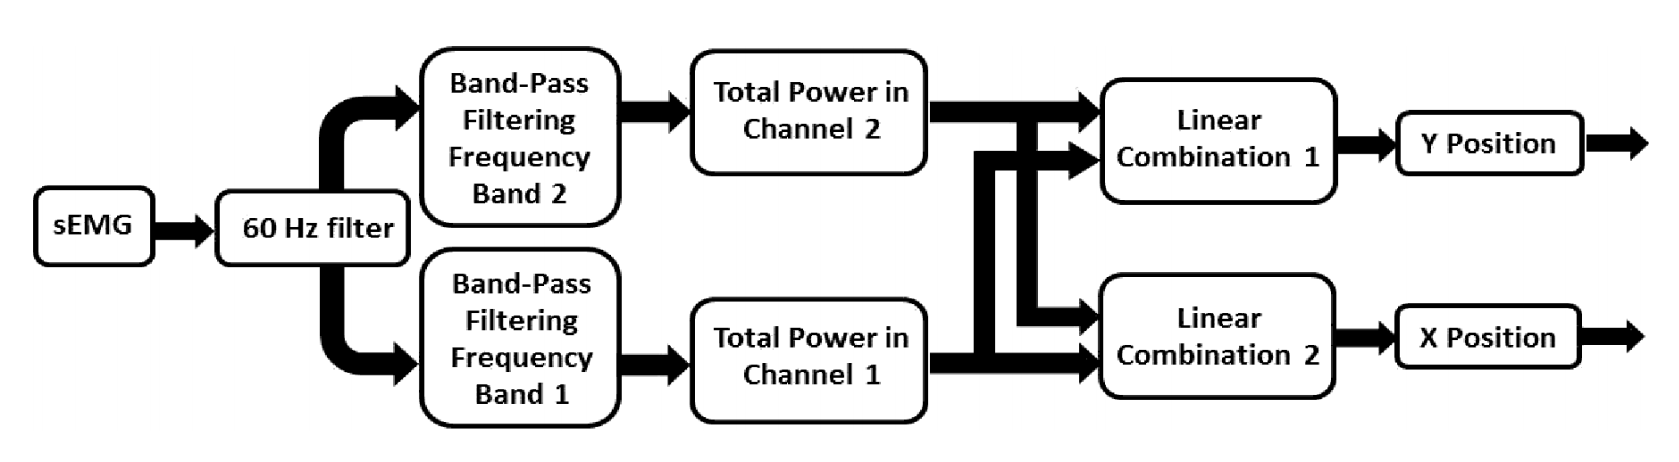
\includegraphics[width=.99\columnwidth]{semg_processing_pipeline.png}
\caption{The single sEMG signal is first processed through a 60 Hz noise filter. It is then run through two different band pass Buttersworth filters to extract two separate signals. The bands are then linearly combined to compute the x and y cursor positions.}
\label{fig:semg_processing_pipeline}
\end{figure}

\subsection{sEMG GUI}
To send signals to the grasping system, the user controls a cursor to hit one of four targets, as illustrated in Figure \ref{fig:semg_ui_blank}. Each target represents a different input options. During grasp planning, they are overlaid on the augmented reality display. The user begins in a rest area and moves the cursor to one of the targets. When the target is hit, the cursor changes colors to reflect the user's selection. The user returns the cursor to the rest area, at which point the input option selected is activated. After a selection, the other targets are disabled for four seconds. If an unintended target is selected, the user can force the selection to \emph{timeout} by avoiding rest for these four seconds, canceling the selection. 

We map these inputs to following a similar strategy to that used for each facial gesture in \emph{System 2}. For the red and green inputs, denoted input 1 and input 2, the input is activated a single time when the user returns to rest. For inputs 3 and 4, the magenta and black targets respectively, the activation is sent continuously until the user exits the rest area again. This allows the user to exert near continuous control over the approach direction. 

\begin{figure}
\centering
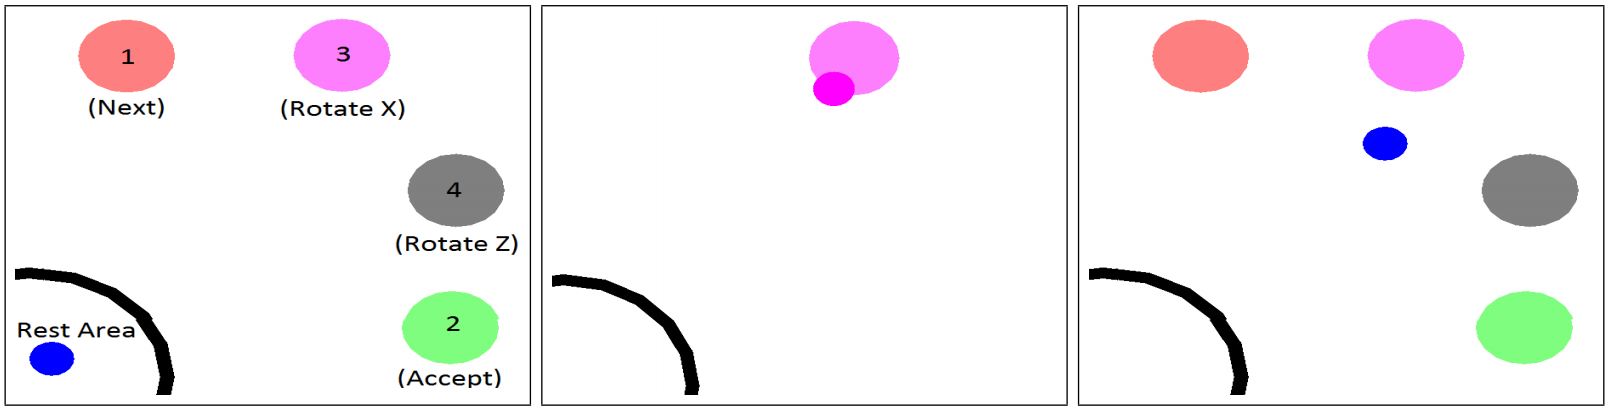
\includegraphics[width=.99\textwidth]{semg_interface_blank.png}
\caption{The sEMG Interface: (a) The user interface is composed of 4 targets overlaid on the grasping scene. Target 1 usually signals acceptance of the current option. Target 2 toggles the next option. Targets 3 and 4 provide input to the planner.(b) Hitting one particular target changes the color of the cursor to reflect the selection and makes the other targets unavailable. (c) If the user does not return to the rest area after a few seconds, the selection times out and is deselected and all targets become available again for selection. }
\label{fig:semg_ui_blank}
\end{figure}


\subsection{Handling Cluttered Scenes}
In addition to an improved input device, we extended our grasping system to handle more realistic scenes, including some amount of clutter. In this work, we will define ``clutter'' as objects being in close enough proximity that many of the grasps for the objects may collide with other nearby objects, but that they are not actually in contact with one another. We did not handle the problem of singulation, which is a specialized manipulation designed to separate objects which are too close together for the fingers to surround the object without colliding with other objects. As such, we tested grasp planning scenes where there was at least 5cm of empty space between each object. 

Handling cluttered scenes brings up a number of challenges. First, it slows down the online planning phase. There are many fewer possible grasps and the obstacles divide the state space into discontinuous regions, which creates more local minima in the value of the quality function, which slows down convergence. Additionally, adding more geometry to the planning scene slows down collision detection, which is a bottleneck for grasp planning. Second, many of the grasps produced by the planner may not have a reachable path to grasp. In our previous systems, we made the optimistic assumption that most grasps were reachable, but in clutter this is no longer a valid assumption. Third, with more objects in the scene, there is more visual clutter and it is more difficult to produce a useful visualization.

In order to address the first two issues, we implemented an online reachability test which the user can clearly interpret. When good grasp candidates are found, \emph{System 3} checks that an entire valid trajectory can be generated using the CBiRRT planner described in \cite{berenson-09}. Unreachable grasps are placed at the end of the list of grasps and colored red in the grasp preview window (see Figure \ref{fig:semg_ui_b}). This allows the user to see that progress is being made even when no new reachable grasps are being generated.

We maintain the list of unreachable grasps so that we can reject nearby grasps without running more computationally expensive analyses. The valid grasps are ranked by their distance to the demonstration hand and alignment to its approach direction. This makes the planner more responsive in cluttered scenes. The list is re-sorted as the demonstration hand is moved.

The results of the reachability test are also used to train a nearest neighbors classifier. When the user moves the demonstration hand, we find the five grasps for which the normal of the palm of the hand is closest to the normal of the demonstrated pose. If at least 50\% of these grasps are unreachable, we designate the current demonstration pose as being in an unreachable region, which is indicated to the user by highlighting the demonstration hand in the planner interface in red. These measures are crucial for a naive user that is not familiar with the kinematics of the robot arm and may not have the intuition that the region they are trying to grasp from is not within the robot's workspace.

\subsection{GUI Modifications For Clutter and sEMG Interface}
 A number of changes were made to the user interface to accommodate both the added visual complexity of overlaying the sEMG control interface on the planning scene and the added difficulty of interpreting the multi-object scene. We redesigned the UI with a cleaner look and feel that implements a number of new features. 

The \emph{System 3} interface layout is outlined in Figure \ref{fig:semg_ui_a}, which illustrates the UI presented during the object selection phase. First, the point cloud displayed in the scene has been upgraded to a higher resolution, color point cloud. This change allows the user to discern the target object more effectively in the cluttered scene. It also allows the user to exercise more judgment in interpreting the scene, since they may not be physically present to observe it first hand. Second, we display only three grasp options instead of 10 to reduce the visual clutter. This also allows us to enlarge the presentation of the grasp so that the user can more easily discern how the hand may interact with the rest of the objects in the scene. Third, we moved the grasp preview window to the side of the screen and modified the way that the UI generates the view to share the aspect ratio and alignment of the depth camera so that all detected objects are visible and that the user's intuition is unimpeded by deformations due to the aspect ratio. Fourth, we removed all of the window decorations and grasp metric displays, as the subject is not expected to be able to interpret them correctly. Overall, this provides a much cleaner, streamlined view more suitable for non-expert users. 

Unfortunately, additional visual clutter is introduced by the addition of the sEMG user interface. This interface is rendered as a translucent layer on top of the grasp planning scene, allowing the subject to see both at the same time. The scene is chosen so that the relevant objects are centered in the scene. While the user is not actively using the cursor it remains in the lower left of the screen and the main grasp planning scene remains unoccluded. 

We placed targets 1 and 2 in opposite corners of the screen because these inputs control the progress of the user through the grasping pipeline, and we wish to minimize confusion between an accidental selection of these two options. The middle two options modify the demonstrated approach direction, and accidental selections have minimal impact. 


\begin{figure}
\centering
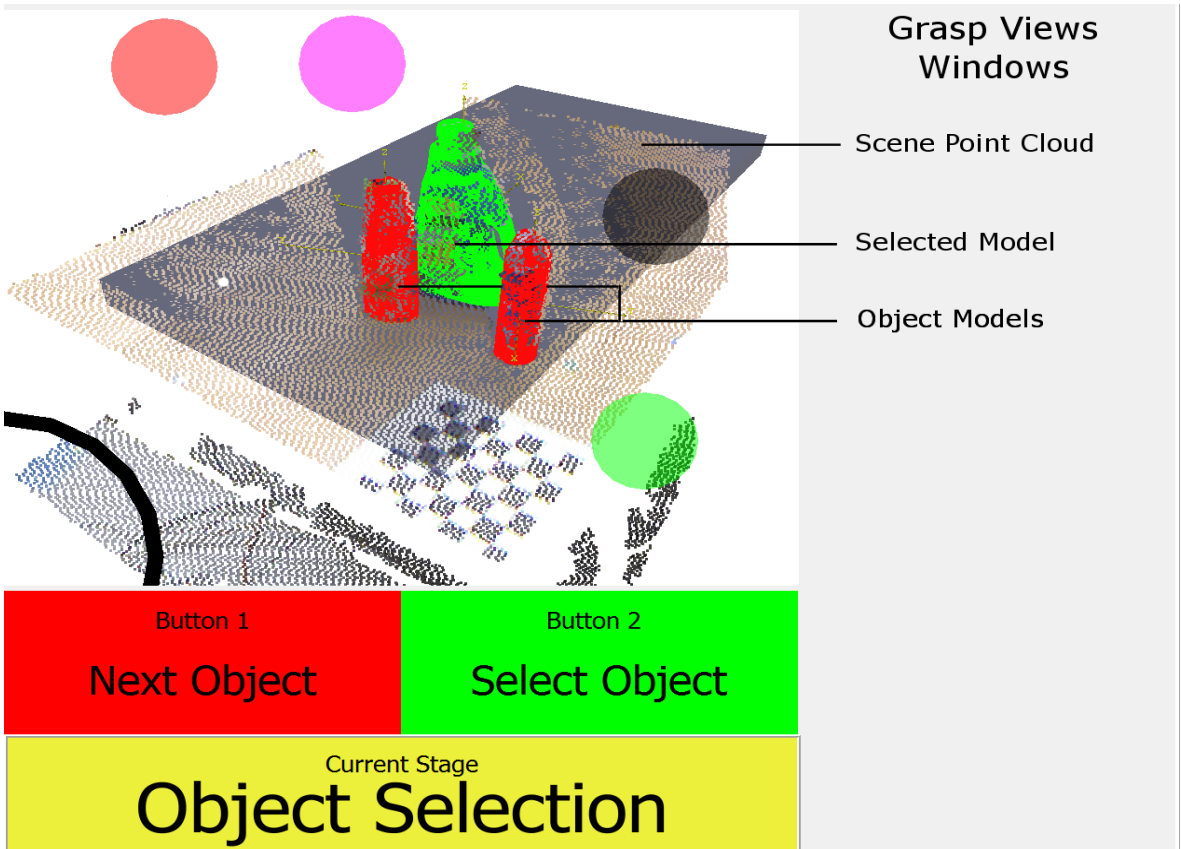
\includegraphics[width=.99\columnwidth]{ui_3_a.png}
\caption{\emph{System 3 Interface - Object Selection Phase.} The subject is able to see the planning scene in the main UI window. The window on the bottom tells the user the current phase and what the green and red inputs will do in this phase. In this phase, the subject sees the point cloud and hits the red target until the object they wish to grasp is highlighted in green. Then they hit the green target to proceed to the next phase.}
\label{fig:semg_ui_a}
\end{figure}

\begin{figure}
\centering
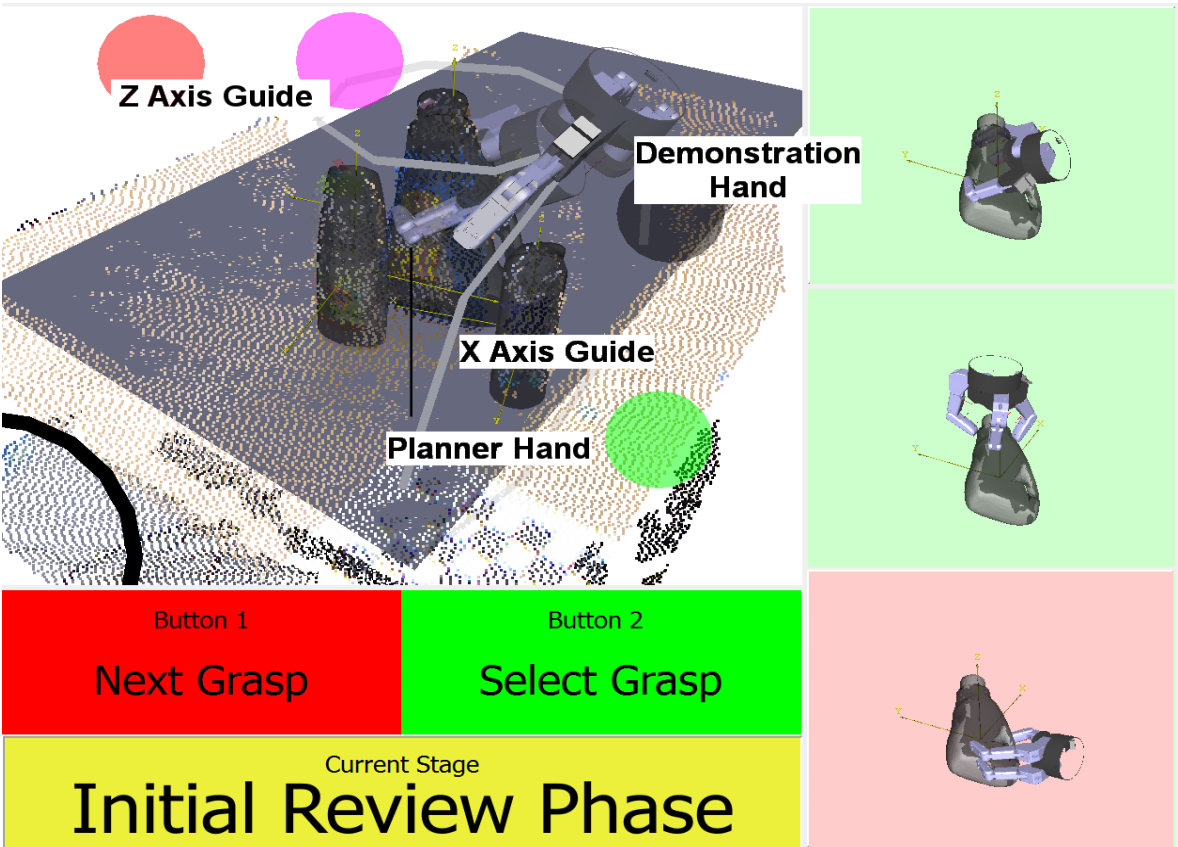
\includegraphics[width=.99\columnwidth]{ui_3_b.png}
\caption{\emph{System 3 Interface - Initial Review Phase.} After the subject selects the object, the Grasp View pane on the right is populated with a set of grasps from a database. Grasps that are reachable appear on a green background, while unreachable grasps are red. A robot hand appears that the user moves to demonstrate a desired starting pose. This demonstration hand is constrained to follow the two circular guides around the z and x axes of the object shown above. The topmost grasp in the grasp view window is the currently selected grasp, which is rendered in the planning scene with the planner hand.}
\label{fig:semg_ui_b}
\end{figure}

\subsection{System 3 Pipeline}
\label{section:pipeline-v3}
\emph{Initialization:} This phase has been modified from \emph{System 2} in that the view is aligned to the true view of the camera, rather than being centered on the target object. This improves the user's overall situational awareness. The user sends input 1 to activate the object recognition system. If the recognized objects align well with the point cloud sent, they can accept the results with input 1. If not, they can rerun the recognition system with input 2.

\emph{Object Selection:} The first detected object is highlighted in green as the target object. To select an object as a target, the user sends input 2. To cycle to the next object in the recognized object list the user sends input 1. The non-target objects are all highlighted in red. The non-target objects are replaced with lower resolution models when a target is selected, which makes the planning phases faster. 

\emph{Initial Review:} As in \emph{System 2}, the user is presented with a list of pre-planned grasps from a precomputed database. This phase has been modified from \emph{System 2} to present the user with a clearer visualization and reachability information. As they iterate through the grasp list, the grasp in the middle and bottom rows shift up and the next grasp in the list moves in to the bottom position. Moving the demonstration hand will also cause the grasp list to re-sort bringing the new approach direction to the top of the list. Reachable grasps are presented on a green background, while unreachable grasps are presented on a red background. The user sends input 1 to increment through the grasp list. When the user finds a reasonable looking grasp, they send input 2 to select the grasp.

\emph{Planner Initialization:} This phase is the same as \emph{System 2}. The user is presented with the choice to either accept the grasp from the third phase with input 1, proceeding straight to the Grasp Choice Confirmation phase or they can send input 2 to refine their chosen grasp further.

\emph{Grasp Refinement:} This phase has been modified from \emph{System 2} to provide feedback about the feasibility of their demonstrated approach direction and grasps. New grasps are displayed with a white background in the grasp preview pane on the right side of the screen while they are being analyzed for reachability. Sending input 2 stops the planner and proceeds to the Final Grasp Review phase.

\emph{Final Grasp Review:} This phase is similar to \emph{System 2}, but adapted to provide more feedback with fewer grasp previews. The user sends input 1 to select the next grasp on the grasp list. They send input 2 to select that grasp. 

\emph{Grasp Choice Confirmation:} The user sends input 1 to go back to the Grasp Refinement phase and input 2 to send the grasp for execution on the robot.


\subsection{Validation}
To validate this system, we recruited a male 30 year old impaired subject with limited upper limb mobility due to a C3-C4 spinal injury. All testing of \emph{System 3} was approved by the Institutional Review Board of the University of California, Davis under Protocol 251192-10. This subject had previous experience with the sEMG device, but had not been trained on this interface. For this work, we measured the activity in the subject's PA muscle to avoid the need to shave the subject's hair. The subject was recruited and trained at the UC Davis site, and operated the robot without ever having any interaction with it or the experiment site in the real world at the Columbia University Robotics Group lab. The setup is shown in Figure \ref{fig:user-semg}. The top of the figure shows the subject with the device attached and using the grasp planning system. The bottom left image is a closeup of the device, which demonstrates how low profile and minimalistic this device is. The bottom right shows the target scene in the robot workspace, with three container objects. The results of this experiment were published in \cite{Weisz2014}, and a video illustrating the experiment can be found at \url{https://youtu.be/tRPXmb9yUbA}.
\begin{figure}
\centering
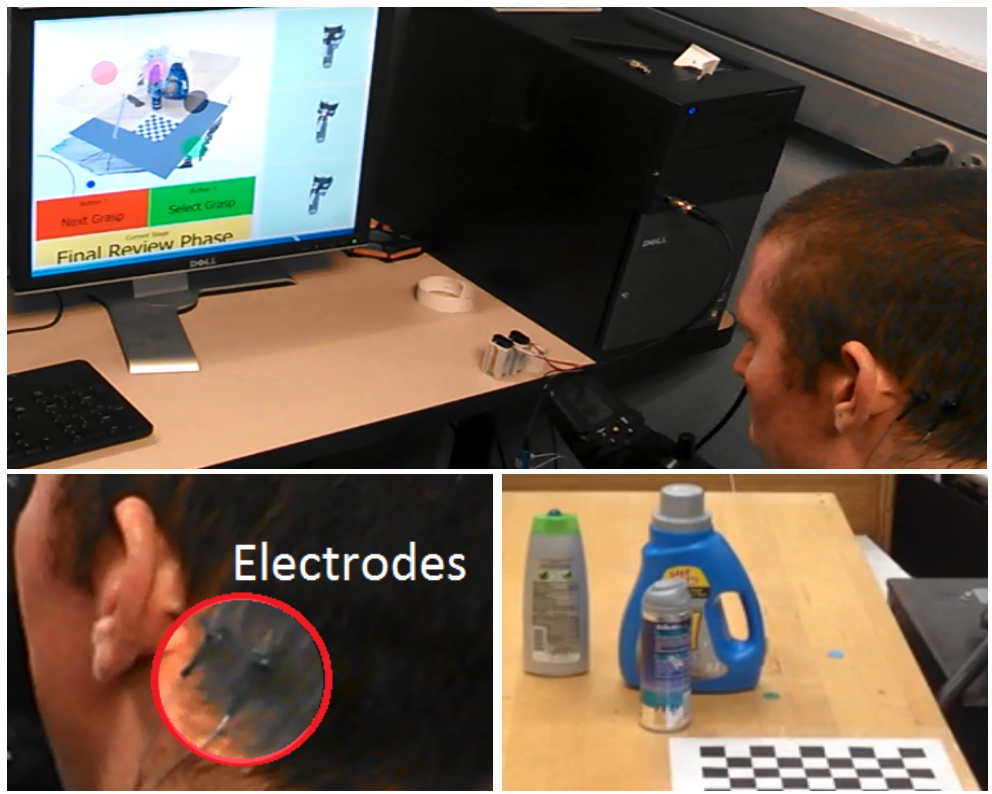
\includegraphics[width=.99\columnwidth]{user_semg.png}
\caption{An impaired subject in the UC Davis RASCAL
lab (top) operating our sEMG-Assistive Grasping interface
to grasp a shaving gel bottle in the Columbia Robotics
Group Laboratory (bottom right). The two small black clips
behind the subject’s ear (bottom left) are surface EMG
electrodes (used in differential mode) to detect activation of
the Posterior Auricular (PA) muscle to direct the system to
pick up the object in this multi-object scene.}
\label{fig:user-semg}
\end{figure}


\subsubsection{Task}
Due to limitations on the impaired subject's time, we were only able to complete three trials using the system. In these three trials,  the subject was asked to pick up an object from a cluttered, multi-object scene. In the first two attempts, he was asked to use the online planner to refine one of the pre-planned grasps. In the first attempt, he grasped the laundry detergent bottle. In the second attempt, he grasped the shaving gel bottle. In the third attempt, he was asked to grasp the detergent bottle using one of the pre-planned grasps directly from the grasp database. Other than the image in the planner interface, the subject was not given any information about the objects he was to grasp. However, they are all well known, household objects, so the subject can be expected to have some implicit idea of the weight and friction properties of the object. 


During the task, the subject reported which target he was trying to reach and we tracked the number of mistaken target activations, which would lead the user to loop back through that part of the pipeline. After the grasp is selected, the target object is lifted off of the table automatically so that the user can see whether the grasp is stable. If no part of the target object remains on the table, we consider the trial a success.

\subsubsection{Training}
To familiarize the subject with the interface, we demonstrated the pipeline two times with the subject just watching and asking questions along the way. We then went through the pipeline with the subject two more times while verbally instructing him on which target to hit while the experimenter controlled the cursor with a computer mouse. This allowed the subject to familiarize himself with the pipeline and navigate their way through it without having to also focus on the task of hitting targets with the sEMG interface. Once he appeared to be conversant with the system, we turned over control to the subject's sEMG interface.

\subsubsection{Results}
The results of the experiment are shown in Tab. \ref{tab:semg_table_1}. The subject was able to grasp the objects successfully on all three attempts. On average, it took the subject 694 seconds to grasp each object, including about 60 seconds for the vision system to detect the objects in the scene. There were an average of 25 timeouts, and 1 mistakenly selected targets per attempt. Timeouts are an expected part of this interface, which allows the user to re-select their intended target if the initially selected target is incorrect. Occasional mistaken selections are also expected, and the pipeline is designed to be robust to these errors, allowing the user to go back to the previous step where necessary to correct mistakes. Several mistakes in a row are necessary to actually realize mistaken actions on the robot.


\begin{table}
\centering
\begin{tabular}{|c|c|c|c|c|}
\hline
Grasp & Time (s) & \#Inputs & \#Timeouts & Mistaken Selections \\ \hline
Detergent 1 & 564 & 14 & 14 & 2\\ \hline
Detergent 2 & 609 & 9 & 50 & 0\\ \hline
Shaving Gel & 910 & 12 & 11 & 1\\ \hline
\end{tabular}
\caption{sEMG Experiment 1 Results}
\label{tab:semg_table_1}
\end{table}

\subsubsection{Discussion}
These results, while promising from the perspective that a single experiment participant was able to understand and utilize the system fairly quickly, demonstrated a number of shortcomings with our system. First, the user's control over the sEMG device was not very accurate, yielding many false initial selections that had to be timed out. This may be because the user was trained to use the PA muscle, which is smaller and has more variable performance. Time restraints did not allow for extensive training of the subject, and so when switching from training to task, the additional cognitive load appears to have degraded performance. A second problem was that the online reachability tester is fairly slow using the CBiRRT planner, and thus new available grasps appeared slowly. This caused relatively few reasonable grasps to be available, and so the user had more trouble because he had to iterate through more grasps which were not reflective of their intent while looking for a reasonable one. While indicating poor regions for grasping by shading the display hand was somewhat effective at helping the user avoid long waits in regions that were doomed to failure, it was not sufficient near border regions where grasps were possible but unlikely because of occlusions. 

\section*{System 4: A practical assistive grasping platform}
\setcounter{subsection}{0}
\renewcommand*{\theHsection}{chX.\the\value{section}}
Our initial results showed enough efficacy of this system that we developed a second prototype using a smaller, lower weight robotic arm, the Kinova Mico. Our initial prototype used an industrial arm, which is extremely accurate and has a large workspace, but is too heavy and expensive to be part of an assistive robotic setup. Additionally, this large, high precision arm does not reflect the performance characteristics of an arm which is affordable and practical for a robotic wheel chair. The Kinova Mico arm is more suitable for mounting on a wheel chair. 
We also sought feedback from our colleagues at the Columbia Medical Center who worked with this same sEMG device in stroke patients. Their advice was that our user interface needed further streamlining. We also sought to resolve the online reachability checking issue by integrating a faster planner. 

\subsection{Adaptations For the Mico Manipulator}
The Kinova Mico arm is a six DOF arm with a two finger gripper. The fingers each have two joints coupled to a passive under-actuation mechanism that enables both enveloping grasps of convex cross sections of objects and fingertip grasps. These fingers are made of a hard plastic which has relatively little friction, which implies that the fingers of the hand must be well aligned to the surface of the object to achieve a stable grasp. 

The transmission of the under-actuation mechanism of the hand is designed such that the fingertips remain at roughly same angle relative to the palm through most of the range of the finger's motion, similar to the motion of a parallel jaw gripper. For hands of this type, we can trivially estimate the contact point of the grasps without performing the kinematic simulation of closing the hand in GraspIt!, which is the most computationally expensive aspect of grasp analysis. In this work, we applied 10x multiplier to the quality measure of grasps whose estimated contacts aligned to within $3^{\circ}$ of the normal to the nearest surface. This was sufficient to generate only well aligned, reasonable grasp candidates. 

%to do this is to add a number of parallel virtual contacts to the grasping surfaces of the finger, as shown in Fig. \ref{fig:mico_finger_virtuals}. Additionally,

\subsection{Improved Online Reachability Checking}
Given our previous insight that the online reachability testing is a bottleneck for the online grasp refinement, we wanted to explore a different options for online reachability checking. This motivated us replace the OpenRave trajectory planner with with the MoveIt! planning environment (see \cite{moveit}), which interfaces with a large number of planners in the OMPL planning library \cite{ompl}.

The OMPL planners have different strategies with different performance properties. In order to investigate which one is appropriate to grasping in the cluttered scenes with the Mico Arm, we captured 10 scenes similar to that in Figure \ref{fig:ui-4-total-a} and ran the online reachability checker on the set of default grasps for each of the objects in the scene. Since many of the grasps in the online planner tend to be very similar, we perturbed the grasps by a +/- 0.005 m in each direction, testing 60 grasps for each of three objects for each scene. 

The online reachability check is the final stage of filtering before grasps are presented to the user. The sampling nature of the planner implies that there will be a great deal of temporal correlation between grasp requests. In order to take advantage of this correlation, we implemented a plan caching scheme which stores the start and end point of the arm trajectory in a nearest neighbors lookup tree. When planning a new trajectory for online analysis, we first attempt to plan from the end of the nearest endpoint. If that fails, we retry from the original starting position. If this second attempt succeeds, the planned path is inserted into the cache. For the actual arm motion, we retry the planning until it succeeds from the original starting location, so long as a valid cached plan exists. This is because smoothing such plans to remove the excess waypoints introduced by the initial segment from the cached plan is still an open area of research that we did not wish to address in this work.  

Because the trajectory planners are stochastic, their performance is highly task specific and sensitive to parameters such as minimum segment length and allowed planning time. We did a parameter sweep of the allowed trajectory segment length from 0.01 to 0.1 in steps of 0.01 with allowed planning times up to 20 seconds. Two of the Probablistic Road Map (PRM) planners (\cite{PRM}) planners performed the best using the caching scheme, succeeding in 43\% of the grasps, and the vanilla PRM implementation had the fastest planning for the caching version of the planner, with an average planning time of 5.5 seconds for arm motions in which the caching fails, and 0.1 seconds when the cache succeeds. 

The single-query bidirectional variant of the PRM planner (SBL) produced plans that seemed smoother in the region near the object. Planning grasps in a cluttered scene is state space in which there is a very narrow valid region near the goal state, and so one might expect a bidirectional planner to find a more optimal path out of that region because it will spend more resources directly on that part of the problem. 

However, we found empirically, when the caching scheme failed to find a reasonable neighbor, the SBL planner's success rate dropped to 30\%, whereas the PRM planner's success rate remained the same. This led to slight lag in performance as the cache was populated. So, for the online reachability verification, we used the PRM planner with a segment length of 0.05, while for producing the actual grasp on the robot we used the SBL planner. These changes removed the online reachability checking as a bottleneck for the online grasp refinement phase of the pipeline. \footnote{Although MoveIt! includes a benchmarking suite for determining the optimal parameters for a set of problems, it cannot be used with MoveIt!'s pick and place grasping pipeline, which handles the approach and lift phases of the path planning, or with robots that have some joints with continuous joint ranges. As such, we implemented our own, less comprehensive optimization script.}

\subsection{Further UI Improvements}
In our previous systems, the two 'continuous' inputs which shifted the hand around the object were not part of the pipeline guide display which showed the user which phase they were in and what their inputs would do. In every phase of the pipeline, they always did the same thing. However, in this system, the purpose of these inputs can also change in each phase. In addition, our previous test user indicated that there should be a clearer differentiation between the augmented reality region containing the grasp planning scene and the rest of the UI and fewer grasp options presented during the parts of the pipeline where they are not needed.

In this system, the UI window is adaptive, providing more visual cues to the user as to what their goal is in each particular phase of the pipeline. The grasp previews are integrated with the pipeline guide display, and the pipeline guide areas also function as GUI buttons for the experimenter to use when familiarizing the subject with the UI. Each of the targets now has a corresponding color coded button. These new UI elements are shown in Figure \ref{fig:ui-4-object-selection} and Figure \ref{fig:ui-4-total-a}. While this may seem like unnecessary complexity, the UI is more visibly different in each phase and less extraneous information is presented. This seems to help subjects keep track of what phase they are in and what its purpose is. 

\begin{figure}
\centering
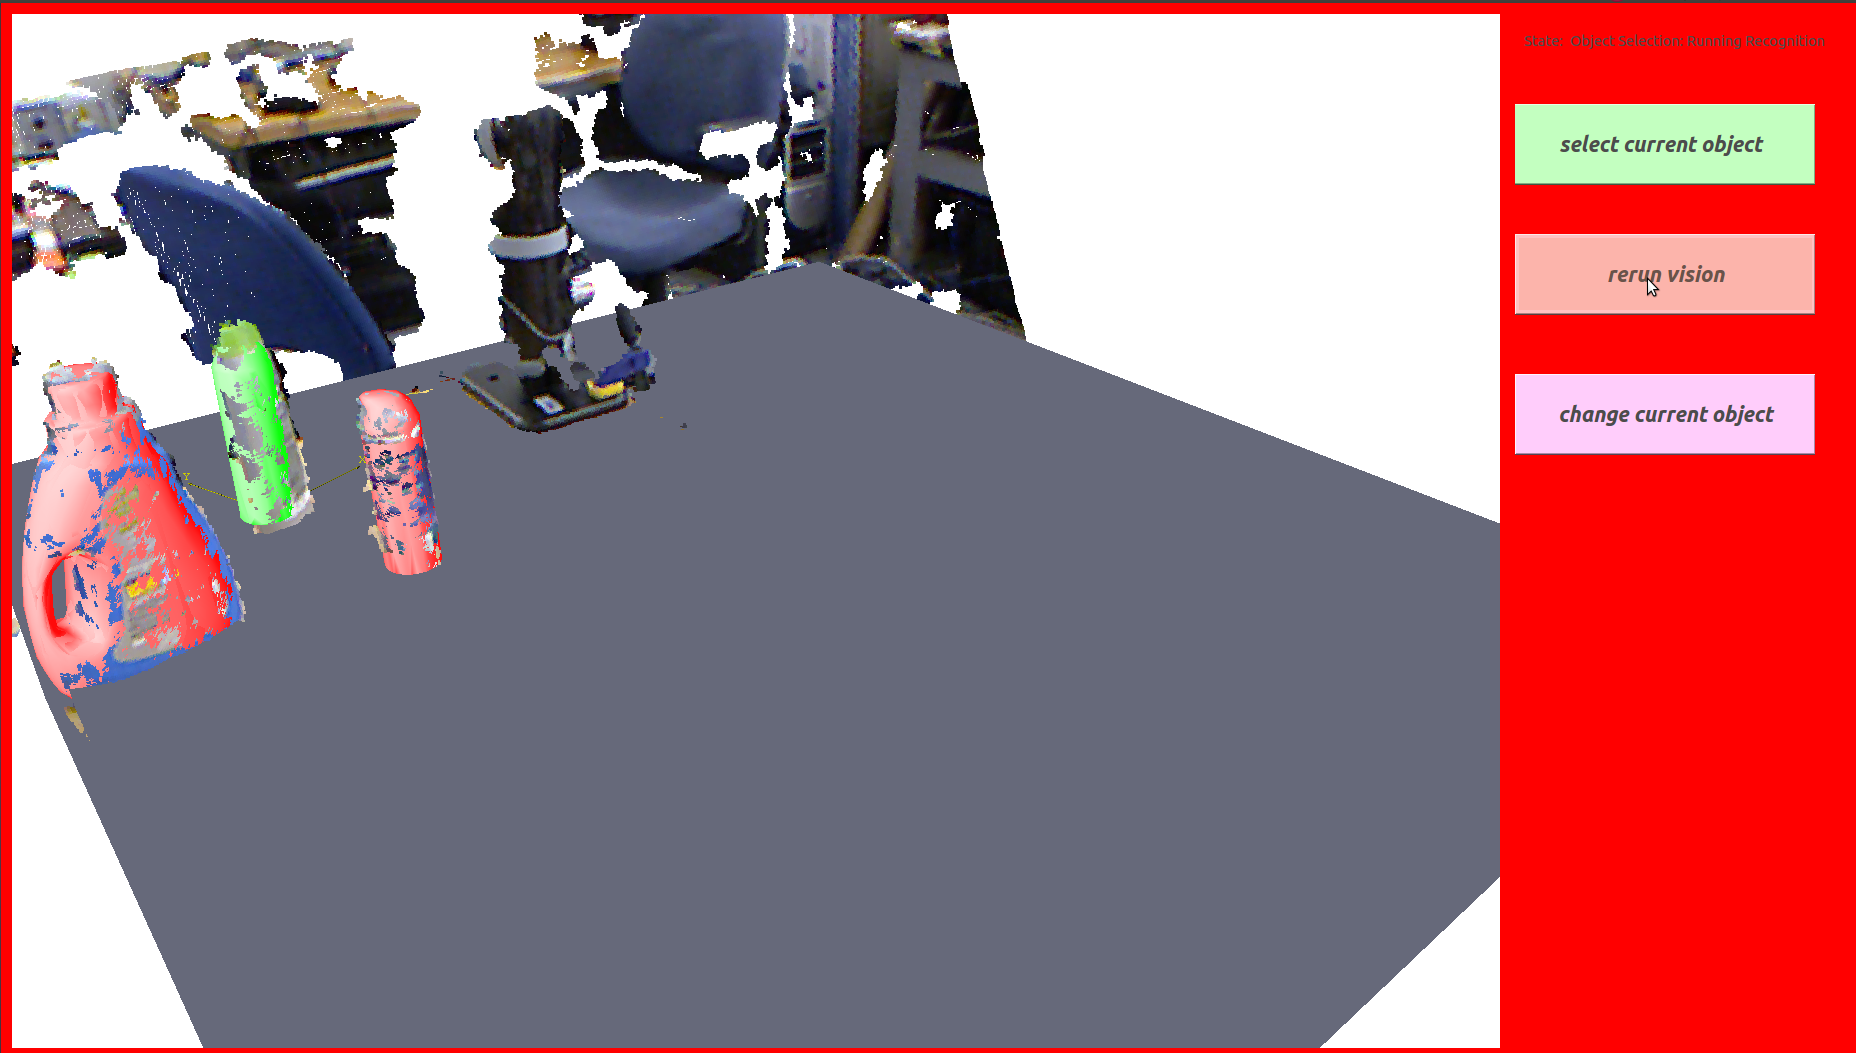
\includegraphics[width=.9\columnwidth]{images_4/object_recognition_state.png}
\caption{\emph{System 4 - Object Recognition and Selection State.} The graspable objects in the seen are highlighted in red and green. Sending input 1 selects the green object as the target, input 2 cycles to the next object, and input 3 triggers the object recognition system to refresh.   The background UI area is rendered in red while the recognition is still processing.}
\label{fig:ui-4-object-selection}
\end{figure}

\subsection*{System 4 Pipeline}
The updated pipeline is slightly shorter and makes more varied use of inputs 3 and 4. 

\emph{Object Recognition and Selection:} This phase combines the first two phases of \emph{System 3}. To select an object as a target, the user sends input 2. To cycle to the next object in the recognized object list the user sends input 3, which will continuously iterate through the grasps until the user leaves the rest area. To rerun the object recognition system the user sends input 1. While the recognition system is still running, the whole screen is highlighted in red and it is not possible to proceed to the next phase until the recognition finishes. 

\emph{Initial Review:} As in the \emph{System 3}, the user is presented with a list of preplanned grasps from a precomputed database. The UI presented is shown in Figure \ref{fig:ui-4-total-a}, in which the currently selected grasp is shown in the window of the top of the guide area, with the color of the background again indicating the results of the online reachability checker. The next grasp is shown in the bottom of the window. Input 1 begins the online refinement stage, input 2 skips to the Final Grasp Review phase. Input 3 will iterate through the available grasps, whereas input 4 will return to the Object Recognition and Selection Phase.

\emph{Grasp Refinement:} This phase is similar to \emph{System 3}, but with one fewer grasp displayed more prominently. The first grasp shown in the top of the window and the next grasp shown on the bottom. Input 1 proceeds to the Final Grasp Review phase, input 2 aligns the hand to the next grasp and brings it up to the top window. Inputs 3 and 4 rotate the hand around the object as previously described. 

\emph{Final Grasp Review:} As in the previous phase, this phase has been adapted to have only two grasps, the top showing the current selection and the bottom showing the next selection. Input 1 proceeds to the Grasp Choice Confirmation phase, input 2 aligns the hand to the next grasp and brings it up to the top window. Inputs 3 and 4 rotate the hand around the object as previously described. 

\emph{Grasp Choice Confirmation:} This phase is similar to \emph{System 3}, but with only the selected grasp shown in the grasp preview window. The user sends input 1 to go back to the Grasp Refinement phase and input 2 to send the grasp for execution on the robot.

\begin{figure}
\centering
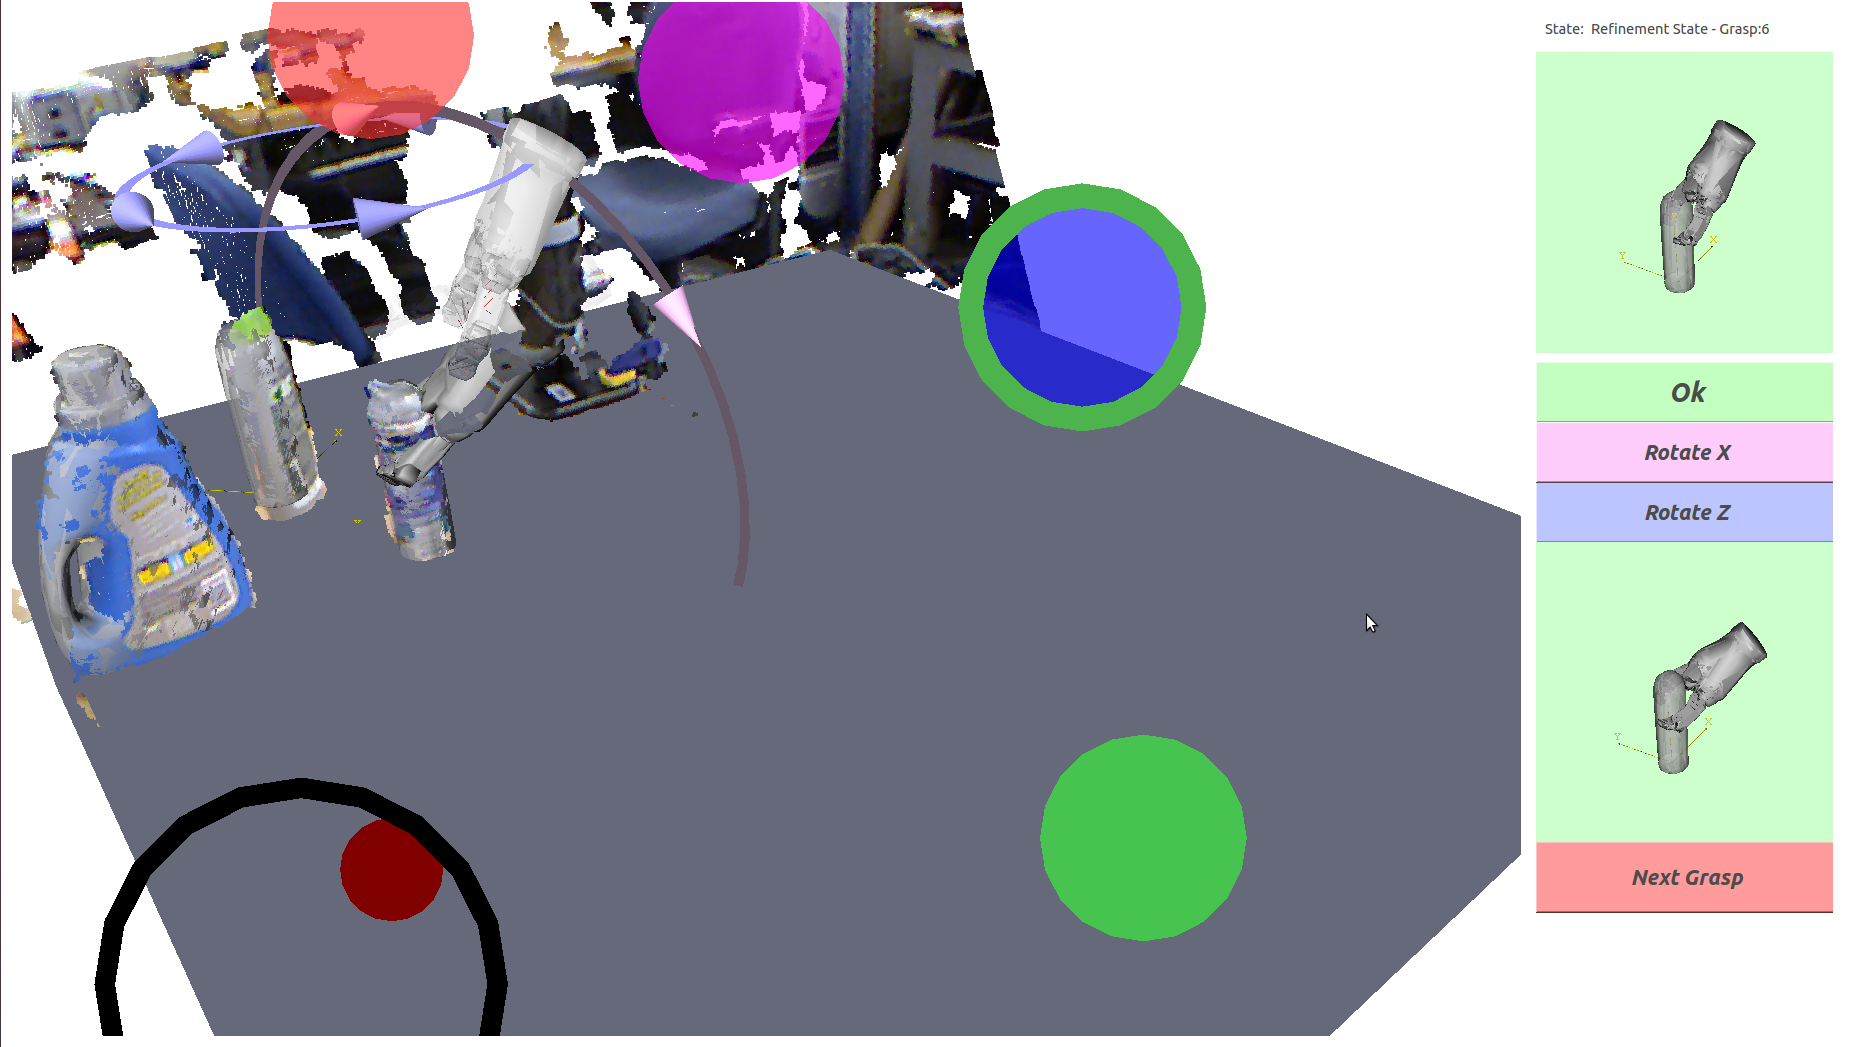
\includegraphics[width=.99\columnwidth]{images_4/matlab_ui.png}
\caption{\emph{System 4 - Grasp Refinement State.} The buttons on the right function as both guides for the result of hitting the color coded input options that will be presented to the use, as well as buttons that the user and experimenter use during the training stage. The sEMG is interface overlaid on the planning scene with the selected target highlighted in green.}
\label{fig:ui-4-total-a}
\end{figure}


\subsection{Validation}
To validate these design decisions, we tested our pipeline on 5 healthy subjects, 2 male and 3 female, ages 22-30. All testing was approved by the Institutional Review Board of the Columbia University under Protocol AAAJ6951. To simplify testing of the UI, we did not attempt to train the subjects on the two dimensional version of the user interface. Instead, the subjects were given a similar user interface, but the cursor is constrained to move towards the target representing the 'selected' input, which is outlined in green as shown in Figure \ref{fig:ui-4-total-a}. In order to switch which target is currently 'selected', the user leaves the rest area and returns to it without hitting a target. This cycles the 'selected' target forward by one. This change allowed us to focus on testing improvements the user interface and grasp planning pipeline without needing the more extensive training necessary to train a subject to achieve full 2D control over the cursor. 

\subsubsection{sEMG Device Setup}

\begin{figure}
\centering
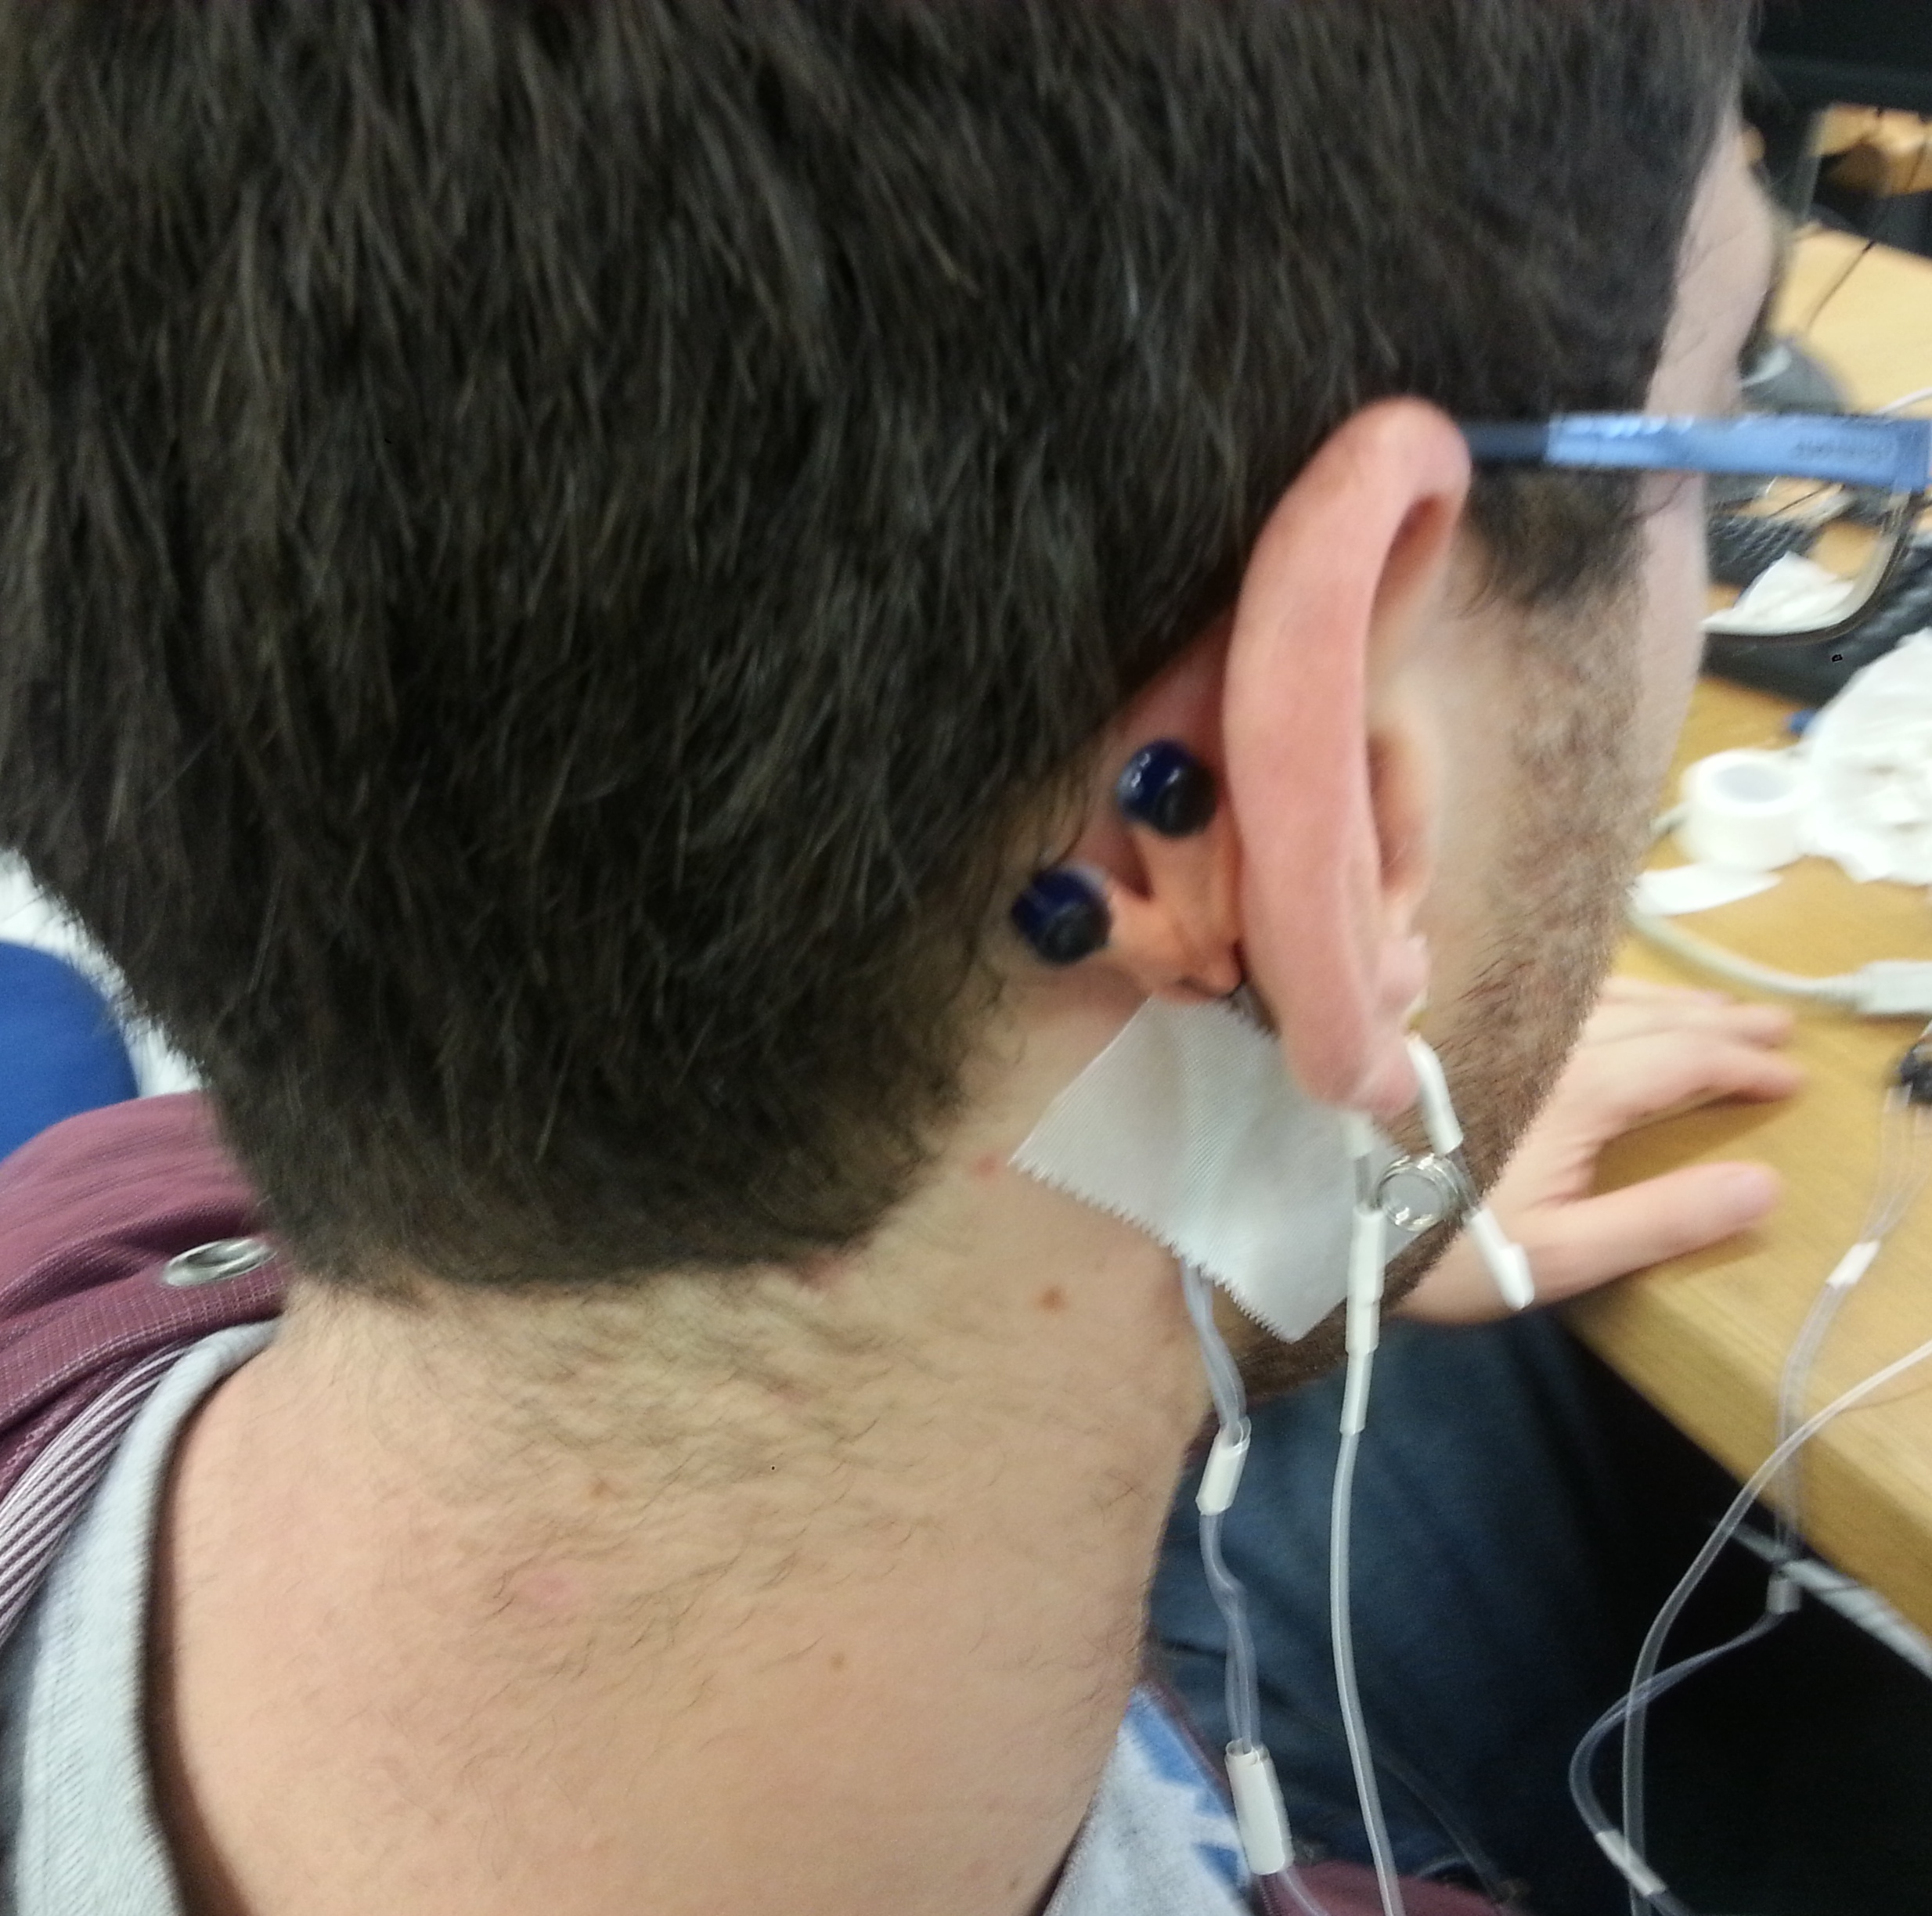
\includegraphics[width=.95\columnwidth,trim={30cm 40cm 20cm 20cm},clip=true]{user_semg_2.jpg}
\caption{The sEMG system electrodes. In these experiments, we placed the electrodes behind the ear of the subject to measure contractions of the PA muscle. We stabilize the electrodes by wrapping the head of the electrodes in Silly Putty silicone putty.}
\label{fig:silly-putty}
\end{figure}

In these experiments, we placed the sEMG device behind the ear of the subject to measure contractions of the PA muscle. In order to stabilize the device and reduce noise due to motion of the wires, we stabilize the electrodes by wrapping the head of the electrodes in Silly Putty\textsuperscript{TM} silicone putty, as shown in Figure \ref{fig:silly-putty}. We find the correct placement of the device by asking the subject to clench their jaw gently and raise their eyebrows. We place the electrodes where we find a large response to eyebrow raises and  little response to jaw motion.

\subsubsection{Training}
\emph{sEMG Device:} Each subject was trained on the sEMG user interface without the grasp planning system. In the training system, the user is given a \emph{desired target} highlighted in red which is randomly selected at the beginning of each trial. The user is then instructed to cycle the \emph{selected target} until it overlaps with the \emph{desired target}, which is then shown in gold. The subject was asked to perform sets of 30 trial blocks until they successfully completed at least 29 of the 30 attempts. This took at most 2 blocks of trials for any subject, with subjects who already had some ability to move their ears frequently succeeding in their first block. 

\emph{Grasp Planning Interface:} To familiarize the subject with the grasp planning system, we manually showed the subject three examples of grasping objects, once short circuiting the online planning and twice allowing the online refinement to run. Then we allowed the subject to guide the pipeline themselves five times, twice without the online planner and three times with it. Then we repeated the training allowing the subject to guide the planner to pick up the large detergent bottle five times in whatever direction they chose using the UI through the on screen button interface. 

\subsubsection{Task}
We placed the objects on the table in proximity to one another as shown in Figure \ref{fig:ui-4-total-a}. We asked the subject to grasp each object three times, the first time from any direction they deemed reasonable, once from the side, and once from above. For each object, the placement of the objects and grasps in the database were such that either the side or top grasp required the online grasp refinement. Since the workspace of the Mico arm is not very large, it is easy to find such object positions. 

\subsubsection{Results}
\label{sec:semg_results}
The results of the experiment for 5 subjects are tabulated in Tab. \ref{tab:results_3}. On average, the subjects were successful in grasping 82\% of the objects within 92 seconds of the first time their cursor left the rest area. With respect to speed,  results are comparable, and indeed somewhat better than the amount of time it took subjects to grasp objects with the Emotiv Epoc, even though the subject may have to iterate over the possible options before selecting them. Subjects 2 and 3 were the best able to control the cursor, having previously been able to move their ears already, and also performed the best in these experiments. These results indicate that the underlying planning system is providing options that the less capable subjects are not exploring because they are having more difficult with the UI. 

For the shampoo bottle, there are relatively fewer grasps that can succeed as compared to the rotationally symmetric shaving gel bottle and the taller, sloping detergent bottle. The only feasible grasps from the side for the shampoo bottle are directly from the side, aligned with the wide axis of the bottle, as demonstrated in Figure \ref{fig:semg-clutter-grasp}. This narrow feasible region and the potential for many collisions with the other objects in the scene during the reaching motion to this region makes this a particularly difficult grasp, especially when the clearance around the grasp is as tight as it is in Figure \ref{fig:semg-clutter-grasp}. Without the partial plan caching implemented in the online trajectory planner, planning grasps to this region using stochastic, sampling based planners is extremely unreliable. With the caching scheme, this grasp was successfully found 100\% of the time, although the planning time is somewhat longer than the other grasp tasks.  

% \singlespace
% \begin{table}[t]
% \raggedleft
% \begin{minipage}[t]{0.4\columnwidth}
% \begin{tabular}[t!]{ | c c c c | }
% \hline
% Grasp & Subject & Success & Time \\ \hline \hline
% \multirow{6}{*}{\begin{minipage}[t]{0.2\columnwidth}Detergent Bottle Top\end{minipage}} & 1 & Yes & 75 \\ 
% & 2 & Yes & 53 \\ 
% & 3 & No & 45 \\
% & 4 & No & 122 \\
% & 5 & Yes & 135 \\ 
% & Mean & 60\% & 86\\\hline
% \multirow{6}{*}{\begin{minipage}[t]{0.2\columnwidth}Detergent Bottle Side\end{minipage}} & 1 & No & 66 \\ 
% & 2 & Yes & 40 \\ 
% & 3 & Yes & 52 \\
% & 4 & Yes & 80 \\
% & 5 & Yes & 85 \\ 
% & Mean & 80\% & 64\\\hline
% \multirow{6}{*}{\begin{minipage}[t]{0.2\columnwidth}Detergent Bottle Open Choice\end{minipage}} & 1 & Yes & 50 \\ 
% & 2 & Yes & 57 \\ 
% & 3 & Yes & 53 \\
% & 4 & Yes & 135 \\
% & 5 & Yes & 128 \\ 
% & Mean & 100\% & 85\\\hline
% \multirow{6}{*}{\begin{minipage}[t]{0.2\columnwidth}Shampoo Bottle Top\end{minipage}} & 1 & Yes & 151 \\ 
% & 2 & Yes & 72 \\ 
% & 3 & Yes & 60\\
% & 4 & No & 126 \\
% & 5 & No & 104 \\ 
% & Mean & 60\% & 102\\\hline
% \multirow{6}{*}{\begin{minipage}[t]{0.2\columnwidth}Shampoo Bottle Side\end{minipage}} & 1 & Yes & 134 \\
% &2 & Yes & 95 \\
% &3 & Yes & 132 \\
% &4 & Yes & 164 \\
% &5 & Yes & 143 \\ 
% & Mean & 100\% & 133\\\hline
% \end{tabular}
% \end{minipage}
% \hspace{.01\columnwidth}
% \raggedright
% \begin{minipage}[!t]{.4\columnwidth}
% \begin{tabular}[t!]{ | c c c c | }
% \hline
% Grasp & Subject & Success & Time \\ \hline \hline
% \multirow{6}{*}{\begin{minipage}[t]{0.2\columnwidth}Shampoo Bottle Open Choice\end{minipage}} & 1 & Yes & 93 \\
% &2 & Yes & 121 \\
% &3 & Yes & 63 \\
% &4 & Yes & 95 \\
% &5 & Yes & 117 \\ 
% & Mean & 100\% & 98\\\hline 
% \multirow{6}{*}{\begin{minipage}[t]{0.2\columnwidth}Shaving Gel Top\end{minipage}} & 1 & No & 83 \\ 
% & 2 & No & 123 \\ 
% & 3 & Yes & 112\\
% & 4 & No & 139 \\
% & 5 & Yes & 97 \\ 
% & Mean & 60\% & 111\\\hline 
% \multirow{6}{*}{\begin{minipage}[t]{0.2\columnwidth}Shaving Gel Side\end{minipage}} & 1 & Yes & 65 \\
% &2 & Yes & 52 \\
% &3 & Yes & 57 \\
% &4 & Yes & 88 \\
% &5 & Yes & 92 \\ 
% & Mean & 100\% & 71\\\hline 
% \multirow{6}{*}{\begin{minipage}[t]{0.2\columnwidth}Shaving Gel Open Choice\end{minipage}} & 1 & No & 73 \\
% &2 & Yes & 59 \\
% &3 & Yes & 76 \\
% &4 & Yes & 81 \\
% &5 & Yes & 85 \\ 
% & Mean & 80\% & 75\\\hline 
% \multirow{6}{*}{\begin{minipage}[t]{0.2\columnwidth}Average Performance\end{minipage}} & 1 & 66\% & 87 \\
% &2 & 88\% & 75 \\
% &3 & 88\% & 72 \\
% &4 & 77\% & 114 \\
% &5 & 88\% &  109\\ 
% & Mean & 82\% & 92\\\hline 
% \end{tabular}
% \end{minipage}
% \caption{Results from Experiment 3. On average, the subjects were successful in grasping 82\% of the objects within 92 seconds of the first time their cursor left rest area.}
% \label{tab:results_3}
% \end{table}
% \doublespace

%\singlespace
\begin{table}[t]
\raggedleft
\begin{minipage}[t]{0.5\columnwidth}
\begin{tabular}[t!]{ | c c c c | }
\hline
Grasp & Subject & Success & Time \\ \hline \hline
\multirow{6}{*}{\begin{minipage}[t]{0.2\columnwidth}Detergent Bottle Top\end{minipage}} & 1 & Yes & 75 \\ 
& 2 & Yes & 53 \\ 
& 3 & No & 45 \\
& 4 & No & 122 \\
& 5 & Yes & 135 \\ 
& Mean & 60\% & 86\\\hline
\multirow{6}{*}{\begin{minipage}[t]{0.2\columnwidth}Detergent Bottle Side\end{minipage}} & 1 & No & 66 \\ 
& 2 & Yes & 40 \\ 
& 3 & Yes & 52 \\
& 4 & Yes & 80 \\
& 5 & Yes & 85 \\ 
& Mean & 80\% & 64\\\hline
\multirow{6}{*}{\begin{minipage}[t]{0.2\columnwidth}Detergent Bottle Open Choice\end{minipage}} & 1 & Yes & 50 \\ 
& 2 & Yes & 57 \\ 
& 3 & Yes & 53 \\
& 4 & Yes & 135 \\
& 5 & Yes & 128 \\ 
& Mean & 100\% & 85\\\hline
\multirow{6}{*}{\begin{minipage}[t]{0.2\columnwidth}Shampoo Bottle Top\end{minipage}} & 1 & Yes & 151 \\ 
& 2 & Yes & 72 \\ 
& 3 & Yes & 60\\
& 4 & No & 126 \\
& 5 & No & 104 \\ 
& Mean & 60\% & 102\\\hline
\multirow{6}{*}{\begin{minipage}[t]{0.2\columnwidth}Shampoo Bottle Side\end{minipage}} & 1 & Yes & 134 \\
&2 & Yes & 95 \\
&3 & Yes & 132 \\
&4 & Yes & 164 \\
&5 & Yes & 143 \\ 
& Mean & 100\% & 133\\\hline
\end{tabular}
\end{minipage}
\hspace{.03\columnwidth}
\raggedright
\begin{minipage}[!t]{.4\columnwidth}
\begin{tabular}[t!]{ | c c c | }
\hline
Grasp & Success & Time \\ \hline \hline
\multirow{6}{*}{\begin{minipage}[t]{0.2\columnwidth}Shampoo Bottle Open Choice\end{minipage}}& Yes & 93 \\
& Yes & 121 \\
& Yes & 63 \\
& Yes & 95 \\
& Yes & 117 \\ 
& 100\% & 98\\\hline 
\multirow{6}{*}{\begin{minipage}[t]{0.2\columnwidth}Shaving Gel Top\end{minipage}} & No & 83 \\ 
& No & 123 \\ 
& Yes & 112\\
& No & 139 \\
& Yes & 97 \\ 
&  60\% & 111\\\hline 
\multirow{6}{*}{\begin{minipage}[t]{0.2\columnwidth}Shaving Gel Side\end{minipage}} & Yes & 65 \\
& Yes & 52 \\
& Yes & 57 \\
& Yes & 88 \\
& Yes & 92 \\ 
& 100\% & 71\\\hline 
\multirow{6}{*}{\begin{minipage}[t]{0.2\columnwidth}Shaving Gel Open Choice\end{minipage}} & No & 73 \\
& Yes & 59 \\
& Yes & 76 \\
& Yes & 81 \\
& Yes & 85 \\ 
& 80\% & 75\\\hline 
\multirow{6}{*}{\begin{minipage}[t]{0.2\columnwidth}Average Performance\end{minipage}} & 66\% & 87 \\
& 88\% & 75 \\
& 88\% & 72 \\
& 77\% & 114 \\
& 88\% &  109\\ 
& 82\% & 92\\\hline 
\end{tabular}
\end{minipage}
\caption{Results from Experiment 3. On average, the subjects were successful in grasping 82\% of the objects within 92 seconds of the first time their cursor left rest area.}
\label{tab:results_3}
\end{table}
%\doublespace


\begin{figure}
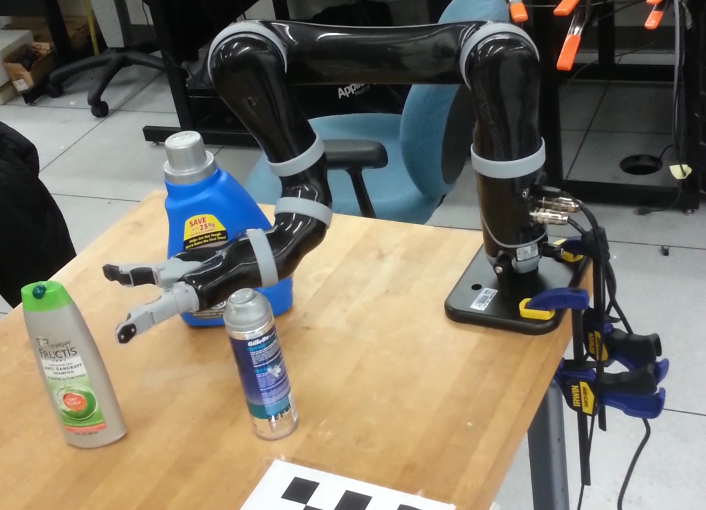
\includegraphics[width=\columnwidth]{images_4/semg_clutter_grasp.png}
\caption{A typical grasp of the shampoo bottle from the side in the cluttered scene. Note that the hand is just able to fit between the other objects to grasp the desired target. Note that the ability to plan this grasp in such a restricted environment is an indication that this system is very successful at handling the cluttered scene.}
\label{fig:semg-clutter-grasp}
\end{figure}

\section{Conclusions}
In this paper, we've discussed the many details involved in building a full assistive grasping system around an online grasp planner. The key challenge was to find the right balance of complexity and usability, particularly with respect to the design of the visual aspects of the interface. A clear user interface is the key to allow a non-expert user to apply their intuition to the grasping problem and provide the added value that makes the system work well in spite of sensor noise and any shortcomings in the heuristics applied by the automated parts of the system. Careful development of this platform has allowed us to produce an extremely capable system around components whose cost and complexity is not prohibitive. 

Through this work with the UC-Davis sEMG device, we have pushed the boundaries of what can be accomplished with a minimally invasive, facial muscle driven input. First, we extended our basic system design to a more complex environment with multiple objects in close proximity to one another. This involved augmenting the user interface with additional phases to select the desired object, adding an online reachability tester, and producing a new UI with a dedicated interface including a cleaner UI with an integrated sEMG driven option selection overlay. After initial validation of the interface on an impaired user, we developed a series of improvements to the user interface, the online grasp planning, and online reachability filter to address the most challenging issues that caused our initial user to take up to eight minutes to make a single grasp selection. We developed a novel control paradigm for testing these changes without changing the visual interface which allowed us to validate the updated system on naive users without the extensive training necessary to train an individual to develop full 2-D control. 

This study serves as a pilot to validate the design choices of the system on a path towards more experiments with impaired users. Even though this paradigm requires the user to make up to four motions for selections which had previously required one, we observed that users took on average 1/8th the time to make grasp selections in the latest version of the sEMG driven planner. We did not explicitly measure how long the users spent in each stage of the pipeline, but one of the most costly phases was observed to be the grasp refinement stage, when it was used. In order to improve performance in this stage, we would have to improve the performance of the collision detection system, which is the dominant cost of the simulated annealing driven grasp refinement. Overall, the majority of the failures to grasp an object were caused by the difficulty of grasping cylinders along the major axis with a gripper, represented by grasping the detergent bottle or shaving gel bottle from above. In these grasps, squeezing the gripper can easily cause the object to be ejected. Subjects cannot seem to learn to expect this behavior without having experienced it a number of times, as they do not have a good sense of the friction properties of the gripper. To improve this behavior, we would have to implement a more complex feedback controller during the grasping process. It is also likely that with greater experience, the subjects would have been more familiar with the kind of grasps that cause ejection. 

This work demonstrates one the first EMG driven grasping systems that we know of that allows a user to grasp an object in a somewhat cluttered scene, or integrates user intent with the intermediate level of control we have proposed. The sEMG device itself is very minimalistic, and could itself be embedded in the frame of a pair of glasses, which makes this device a real candidate for evolving to a consumer level product. Future work for this paradigm will be to refine the training paradigm to make learning 2D control over the device easier, exploring new control paradigms, and extending the user interface to control the locomotion of a motorized wheel chair or mobile manipulator assistive platform. We have also begun some exploration towards more complex grasp quality measures that integrate more complex artificial intelligence techniques such as ``deep learning'' which may have less reliance on the accuracy of the object recognition system. 
